\documentclass[twocolumn]{article}
\usepackage[margin=2cm]{geometry}
\usepackage{tikz,lipsum,amsmath,amssymb,mathrsfs,soul,xcolor,cancel,esint,graphicx}
\tikzset{every picture/.style={line width=0.75pt}} %set default line width to 0.75pt        
\numberwithin{equation}{section}

\NewDocumentCommand{\caja}{ m O{gray!40} O{gray!10} m }{
	\begin{figure}[h]
		\centering
		\begin{tikzpicture}
			\node[anchor=text, text width=\columnwidth-1.2cm, draw, rounded corners, line width=1pt, fill=#3, inner sep=5mm] (big) {\\#4};
			\node[draw, rounded corners, line width=.5pt, fill=#2, anchor=west, xshift=5mm] (small) at (big.north west) {#1};
		\end{tikzpicture}
	\end{figure}
}

\newcommand{\deriv}[3]{\left(\frac{\partial #1}{\partial #2} \right)_{#3}}

\newcommand{\dderiv}[3]{\left(\dfrac{\partial #1}{\partial #2} \right)_{#3}}

\NewDocumentCommand{\indUpDown}{ O{\Lambda} O{\mu} O{\nu} }{
	{#1}^{#2}_{\ #3}
}
\NewDocumentCommand{\indDownUp}{ O{\Lambda} O{\mu} O{\nu} }{
	{#1}_{#2}^{\ #3}
}

\newcommand{\LambdaMuNu}{\indUpDown}
\newcommand{\0}{\textcolor{gray}{0}}
\newcommand{\ei}{\mathbf{e}_i}
\newcommand{\ej}{\mathbf{e}_j}
\newcommand{\lc}{\epsilon_{ijk}}
\newcommand{\gr}{\nabla}
\newcommand{\di}{\nabla\cdot}
\newcommand{\ro}{\nabla\times}
\newcommand{\la}{\nabla^2}
\newcommand{\rv}{\mathbf{r}}
\newcommand{\pv}{\mathbf{p}}
\newcommand{\xv}{\mathbf{x}}
\newcommand{\yv}{\mathbf{y}}
\newcommand{\zv}{\mathbf{z}}
\newcommand{\xhat}{\hat{\xv}}
\newcommand{\yhat}{\hat{\yv}}
\newcommand{\zhat}{\hat{\zv}}
\newcommand{\ihat}{\hat{\mathbf{i}}}
\newcommand{\jhat}{\hat{\mathbf{j}}}
\newcommand{\khat}{\hat{\mathbf{k}}}
\newcommand{\rhat}{\hat{\rv}}
\newcommand{\that}{\hat{\mathbf{\theta}}}
\newcommand{\phat}{\hat{\mathbf{\varphi}}}
\newcommand{\rhhat}{\hat{\mathbf{\rho}}}
\newcommand{\nhat}{\hat{\mathbf{n}}}
\newcommand{\Rhat}{\hat{\mathbf{R}}}
\newcommand{\eo}{\epsilon_{0}}
\newcommand{\uo}{\mu_{0}}
\NewDocumentCommand{\ke}{ O{1}}{
	\frac{#1}{4\pi\eo}
}
\NewDocumentCommand{\ku}{ O{}}{
	\frac{\uo #1}{4\pi}
}
%\newcommand{\ke}{\frac{1}{4\pi\eo}}
%\newcommand{\ku}{\frac{\uo}{4\pi}}
\newcommand{\rdif}{\rv - \rv'}
\newcommand{\pd}[2]{\dfrac{\partial #1}{\partial #2}}
\newcommand{\lpd}[2]{\partial #1/\partial #2}
\newcommand{\spd}[2]{\frac{\partial #1}{\partial #2}}
\newcommand{\td}[2]{\dfrac{d #1}{d #2}}
\newcommand{\ltd}[2]{d #1/d #2}
\newcommand{\std}[2]{\frac{d #1}{d #2}}
\newcommand{\n}[1]{\mathbf{#1}}
\newcommand{\eff}[1]{#1_\mathrm{eff}}
\newcommand{\Ueff}{\eff{U}}

\newcommand{\wfrac}[3][3pt]{%
	\frac{\wfracterm{depth}{\dp}{#1}{#2}}{\wfracterm{height}{\ht}{#1}{#3}}%
}
\newcommand{\wfracterm}[4]{%
	\sbox0{$\displaystyle#4$}%
	\vrule width 0pt #1 \dimexpr #20+#3\relax
	\usebox{0}%
}

\newcommand{\pr}[1]{\left\langle #1 \right\rangle }

\newcommand{\qed}{\hfill\(\blacksquare\)}
\newcommand{\resp}{
	\\
	
	\textbf{Respuesta:} }
\newcommand{\celsius}{^\circ\mathrm{C}}

%opening
\title{Resumen de \textit{Observation of Dirac monopoles in a synthetic magnetic field}}
\author{Simon Fonseca}
\date{}

\begin{document}
	\maketitle
	\section{Referencia completa}
	\textbf{Autores:} M. W. Ray, E. Ruokokoski, S. Kandel, M. Möttönen \& D. S. Hall.
	\textbf{Título:} \textit{Observation of Dirac monopoles in a synthetic magnetic field} (Observación de monopolos de Dirac en un campo magnético sintético).
	\textbf{Revista:} Nature.
	\textbf{Volumen:} 505.
	\textbf{Páginas:} 657–660.
	\textbf{Fecha de publicación:} 30 de enero de 2014.
	\textbf{DOI:} 10.1038/nature12954.
	
	\section{Problema físico}
	\subsection{Monopolos de Dirac}
	Los monopolos magnéticos son partículas que se comportan como polos (norte o sur) magnéticos aislados. Para que estos existan se requeriría que se cumpliese
	\begin{equation}
		\di\n{B} = \rho_M ~\Rightarrow~ \n{B} = \frac{g}{r^2}\rhat \label{B_rho}
	\end{equation}
	donde $\rho_M$ y $g$ son una cierta densidad y carga magnética, respectivamente. Pero la teoría de electrodinámica clásica famosamente no los incluye, una de las leyes de Maxwell nos dice, en cambio, que
	\begin{equation}
		\di\n{B} = 0 ~\Leftrightarrow~ \n{B} = \ro\n{A} \label{B_0}
	\end{equation}
	es decir, la existencia de un monopolo magnético se contradice con la noción de un potencial vectorial $\n{A}$ bien definido en todo el espacio.
	
	Paul Dirac postuló la existencia de monopolos magnéticos en 1931 al relajar la condición sobre el potencial $\n{A}$. Si imaginamos un solenoide semi-infinito de ancho infinitesimal que lleva flujo  magnético desde el infinito hasta un punto arbitrario, lo que tendremos en la práctica es un monopolo magnético en el punto de salida del solenoide.
	
	\begin{figure}[h!]
		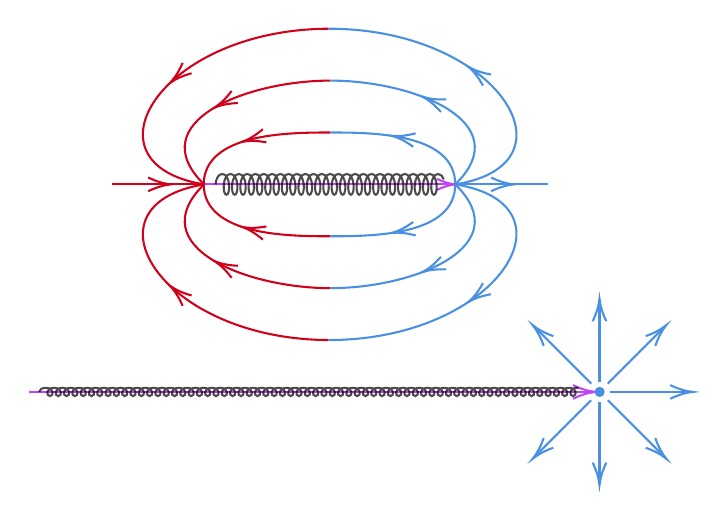
\begin{tikzpicture}[x=0.75pt,y=0.75pt,yscale=-1,xscale=1]
			%uncomment if require: \path (0,300); %set diagram left start at 0, and has height of 300
			
			%Straight Lines [id:da18687793493999383] 
			\draw [color={rgb, 255:red, 193; green, 70; blue, 241 }  ,draw opacity=1 ]   (15,195) -- (286.17,195) ;
			\draw [shift={(288.17,195)}, rotate = 180] [color={rgb, 255:red, 193; green, 70; blue, 241 }  ,draw opacity=1 ][line width=0.75]    (10.93,-3.29) .. controls (6.95,-1.4) and (3.31,-0.3) .. (0,0) .. controls (3.31,0.3) and (6.95,1.4) .. (10.93,3.29)   ;
			%Shape: Spring [id:dp9313734346311904] 
			\draw  [color={rgb, 255:red, 0; green, 0; blue, 0 }  ,draw opacity=0.7 ] (20,195) .. controls (20.25,194) and (21.25,193) .. (23.25,193) .. controls (27.25,193) and (27.25,197) .. (25.25,197) .. controls (23.25,197) and (23.25,193) .. (27.25,193) .. controls (31.25,193) and (31.25,197) .. (29.25,197) .. controls (27.25,197) and (27.25,193) .. (31.25,193) .. controls (35.25,193) and (35.25,197) .. (33.25,197) .. controls (31.25,197) and (31.25,193) .. (35.25,193) .. controls (39.25,193) and (39.25,197) .. (37.25,197) .. controls (35.25,197) and (35.25,193) .. (39.25,193) .. controls (43.25,193) and (43.25,197) .. (41.25,197) .. controls (39.25,197) and (39.25,193) .. (43.25,193) .. controls (47.25,193) and (47.25,197) .. (45.25,197) .. controls (43.25,197) and (43.25,193) .. (47.25,193) .. controls (51.25,193) and (51.25,197) .. (49.25,197) .. controls (47.25,197) and (47.25,193) .. (51.25,193) .. controls (55.25,193) and (55.25,197) .. (53.25,197) .. controls (51.25,197) and (51.25,193) .. (55.25,193) .. controls (59.25,193) and (59.25,197) .. (57.25,197) .. controls (55.25,197) and (55.25,193) .. (59.25,193) .. controls (63.25,193) and (63.25,197) .. (61.25,197) .. controls (59.25,197) and (59.25,193) .. (63.25,193) .. controls (67.25,193) and (67.25,197) .. (65.25,197) .. controls (63.25,197) and (63.25,193) .. (67.25,193) .. controls (71.25,193) and (71.25,197) .. (69.25,197) .. controls (67.25,197) and (67.25,193) .. (71.25,193) .. controls (75.25,193) and (75.25,197) .. (73.25,197) .. controls (71.25,197) and (71.25,193) .. (75.25,193) .. controls (79.25,193) and (79.25,197) .. (77.25,197) .. controls (75.25,197) and (75.25,193) .. (79.25,193) .. controls (83.25,193) and (83.25,197) .. (81.25,197) .. controls (79.25,197) and (79.25,193) .. (83.25,193) .. controls (87.25,193) and (87.25,197) .. (85.25,197) .. controls (83.25,197) and (83.25,193) .. (87.25,193) .. controls (91.25,193) and (91.25,197) .. (89.25,197) .. controls (87.25,197) and (87.25,193) .. (91.25,193) .. controls (95.25,193) and (95.25,197) .. (93.25,197) .. controls (91.25,197) and (91.25,193) .. (95.25,193) .. controls (99.25,193) and (99.25,197) .. (97.25,197) .. controls (95.25,197) and (95.25,193) .. (99.25,193) .. controls (103.25,193) and (103.25,197) .. (101.25,197) .. controls (99.25,197) and (99.25,193) .. (103.25,193) .. controls (107.25,193) and (107.25,197) .. (105.25,197) .. controls (103.25,197) and (103.25,193) .. (107.25,193) .. controls (111.25,193) and (111.25,197) .. (109.25,197) .. controls (107.25,197) and (107.25,193) .. (111.25,193) .. controls (115.25,193) and (115.25,197) .. (113.25,197) .. controls (111.25,197) and (111.25,193) .. (115.25,193) .. controls (119.25,193) and (119.25,197) .. (117.25,197) .. controls (115.25,197) and (115.25,193) .. (119.25,193) .. controls (123.25,193) and (123.25,197) .. (121.25,197) .. controls (119.25,197) and (119.25,193) .. (123.25,193) .. controls (127.25,193) and (127.25,197) .. (125.25,197) .. controls (123.25,197) and (123.25,193) .. (127.25,193) .. controls (131.25,193) and (131.25,197) .. (129.25,197) .. controls (127.25,197) and (127.25,193) .. (131.25,193) .. controls (135.25,193) and (135.25,197) .. (133.25,197) .. controls (131.25,197) and (131.25,193) .. (135.25,193) .. controls (139.25,193) and (139.25,197) .. (137.25,197) .. controls (135.25,197) and (135.25,193) .. (139.25,193) .. controls (143.25,193) and (143.25,197) .. (141.25,197) .. controls (139.25,197) and (139.25,193) .. (143.25,193) .. controls (147.25,193) and (147.25,197) .. (145.25,197) .. controls (143.25,197) and (143.25,193) .. (147.25,193) .. controls (151.25,193) and (151.25,197) .. (149.25,197) .. controls (147.25,197) and (147.25,193) .. (151.25,193) .. controls (155.25,193) and (155.25,197) .. (153.25,197) .. controls (151.25,197) and (151.25,193) .. (155.25,193) .. controls (159.25,193) and (159.25,197) .. (157.25,197) .. controls (155.25,197) and (155.25,193) .. (159.25,193) .. controls (163.25,193) and (163.25,197) .. (161.25,197) .. controls (159.25,197) and (159.25,193) .. (163.25,193) .. controls (167.25,193) and (167.25,197) .. (165.25,197) .. controls (163.25,197) and (163.25,193) .. (167.25,193) .. controls (171.25,193) and (171.25,197) .. (169.25,197) .. controls (167.25,197) and (167.25,193) .. (171.25,193) .. controls (175.25,193) and (175.25,197) .. (173.25,197) .. controls (171.25,197) and (171.25,193) .. (175.25,193) .. controls (179.25,193) and (179.25,197) .. (177.25,197) .. controls (175.25,197) and (175.25,193) .. (179.25,193) .. controls (183.25,193) and (183.25,197) .. (181.25,197) .. controls (179.25,197) and (179.25,193) .. (183.25,193) .. controls (187.25,193) and (187.25,197) .. (185.25,197) .. controls (183.25,197) and (183.25,193) .. (187.25,193) .. controls (191.25,193) and (191.25,197) .. (189.25,197) .. controls (187.25,197) and (187.25,193) .. (191.25,193) .. controls (195.25,193) and (195.25,197) .. (193.25,197) .. controls (191.25,197) and (191.25,193) .. (195.25,193) .. controls (199.25,193) and (199.25,197) .. (197.25,197) .. controls (195.25,197) and (195.25,193) .. (199.25,193) .. controls (203.25,193) and (203.25,197) .. (201.25,197) .. controls (199.25,197) and (199.25,193) .. (203.25,193) .. controls (207.25,193) and (207.25,197) .. (205.25,197) .. controls (203.25,197) and (203.25,193) .. (207.25,193) .. controls (211.25,193) and (211.25,197) .. (209.25,197) .. controls (207.25,197) and (207.25,193) .. (211.25,193) .. controls (215.25,193) and (215.25,197) .. (213.25,197) .. controls (211.25,197) and (211.25,193) .. (215.25,193) .. controls (219.25,193) and (219.25,197) .. (217.25,197) .. controls (215.25,197) and (215.25,193) .. (219.25,193) .. controls (223.25,193) and (223.25,197) .. (221.25,197) .. controls (219.25,197) and (219.25,193) .. (223.25,193) .. controls (227.25,193) and (227.25,197) .. (225.25,197) .. controls (223.25,197) and (223.25,193) .. (227.25,193) .. controls (231.25,193) and (231.25,197) .. (229.25,197) .. controls (227.25,197) and (227.25,193) .. (231.25,193) .. controls (235.25,193) and (235.25,197) .. (233.25,197) .. controls (231.25,197) and (231.25,193) .. (235.25,193) .. controls (239.25,193) and (239.25,197) .. (237.25,197) .. controls (235.25,197) and (235.25,193) .. (239.25,193) .. controls (243.25,193) and (243.25,197) .. (241.25,197) .. controls (239.25,197) and (239.25,193) .. (243.25,193) .. controls (247.25,193) and (247.25,197) .. (245.25,197) .. controls (243.25,197) and (243.25,193) .. (247.25,193) .. controls (251.25,193) and (251.25,197) .. (249.25,197) .. controls (247.25,197) and (247.25,193) .. (251.25,193) .. controls (255.25,193) and (255.25,197) .. (253.25,197) .. controls (251.25,197) and (251.25,193) .. (255.25,193) .. controls (259.25,193) and (259.25,197) .. (257.25,197) .. controls (255.25,197) and (255.25,193) .. (259.25,193) .. controls (263.25,193) and (263.25,197) .. (261.25,197) .. controls (259.25,197) and (259.25,193) .. (263.25,193) .. controls (267.25,193) and (267.25,197) .. (265.25,197) .. controls (263.25,197) and (263.25,193) .. (267.25,193) .. controls (271.25,193) and (271.25,197) .. (269.25,197) .. controls (267.25,197) and (267.25,193) .. (271.25,193) .. controls (275.25,193) and (275.25,197) .. (273.25,197) .. controls (271.25,197) and (271.25,193) .. (275.25,193) .. controls (279.25,193) and (279.25,197) .. (277.25,197) .. controls (275.25,197) and (275.25,193) .. (279.25,193) .. controls (279.46,193) and (279.65,193.01) .. (279.84,193.03) ;
			%Shape: Circle [id:dp9976515953764042] 
			\draw  [color={rgb, 255:red, 74; green, 144; blue, 226 }  ,draw opacity=1 ][fill={rgb, 255:red, 74; green, 144; blue, 226 }  ,fill opacity=1 ] (288.17,195) .. controls (288.17,193.94) and (289.02,193.08) .. (290.08,193.08) .. controls (291.14,193.08) and (292,193.94) .. (292,195) .. controls (292,196.06) and (291.14,196.92) .. (290.08,196.92) .. controls (289.02,196.92) and (288.17,196.06) .. (288.17,195) -- cycle ;
			%Straight Lines [id:da9803337688140109] 
			\draw [color={rgb, 255:red, 74; green, 144; blue, 226 }  ,draw opacity=1 ]   (290,190) -- (290,152) ;
			\draw [shift={(290,150)}, rotate = 90] [color={rgb, 255:red, 74; green, 144; blue, 226 }  ,draw opacity=1 ][line width=0.75]    (10.93,-3.29) .. controls (6.95,-1.4) and (3.31,-0.3) .. (0,0) .. controls (3.31,0.3) and (6.95,1.4) .. (10.93,3.29)   ;
			%Straight Lines [id:da02594517737390256] 
			\draw [color={rgb, 255:red, 74; green, 144; blue, 226 }  ,draw opacity=1 ]   (290,200) -- (290,238) ;
			\draw [shift={(290,240)}, rotate = 270] [color={rgb, 255:red, 74; green, 144; blue, 226 }  ,draw opacity=1 ][line width=0.75]    (10.93,-3.29) .. controls (6.95,-1.4) and (3.31,-0.3) .. (0,0) .. controls (3.31,0.3) and (6.95,1.4) .. (10.93,3.29)   ;
			%Straight Lines [id:da856741703681731] 
			\draw [color={rgb, 255:red, 74; green, 144; blue, 226 }  ,draw opacity=1 ]   (295,195) -- (333,195) ;
			\draw [shift={(335,195)}, rotate = 180] [color={rgb, 255:red, 74; green, 144; blue, 226 }  ,draw opacity=1 ][line width=0.75]    (10.93,-3.29) .. controls (6.95,-1.4) and (3.31,-0.3) .. (0,0) .. controls (3.31,0.3) and (6.95,1.4) .. (10.93,3.29)   ;
			%Straight Lines [id:da6378559154003527] 
			\draw [color={rgb, 255:red, 74; green, 144; blue, 226 }  ,draw opacity=1 ]   (294,199) -- (320.87,225.87) ;
			\draw [shift={(322.28,227.28)}, rotate = 225] [color={rgb, 255:red, 74; green, 144; blue, 226 }  ,draw opacity=1 ][line width=0.75]    (10.93,-3.29) .. controls (6.95,-1.4) and (3.31,-0.3) .. (0,0) .. controls (3.31,0.3) and (6.95,1.4) .. (10.93,3.29)   ;
			%Straight Lines [id:da5620212525131404] 
			\draw [color={rgb, 255:red, 74; green, 144; blue, 226 }  ,draw opacity=1 ]   (294,191) -- (320.87,164.13) ;
			\draw [shift={(322.28,162.72)}, rotate = 135] [color={rgb, 255:red, 74; green, 144; blue, 226 }  ,draw opacity=1 ][line width=0.75]    (10.93,-3.29) .. controls (6.95,-1.4) and (3.31,-0.3) .. (0,0) .. controls (3.31,0.3) and (6.95,1.4) .. (10.93,3.29)   ;
			%Straight Lines [id:da915339395493542] 
			\draw [color={rgb, 255:red, 74; green, 144; blue, 226 }  ,draw opacity=1 ]   (286,199) -- (259.13,225.87) ;
			\draw [shift={(257.72,227.28)}, rotate = 315] [color={rgb, 255:red, 74; green, 144; blue, 226 }  ,draw opacity=1 ][line width=0.75]    (10.93,-3.29) .. controls (6.95,-1.4) and (3.31,-0.3) .. (0,0) .. controls (3.31,0.3) and (6.95,1.4) .. (10.93,3.29)   ;
			%Straight Lines [id:da061391798493468874] 
			\draw [color={rgb, 255:red, 74; green, 144; blue, 226 }  ,draw opacity=1 ]   (286,191) -- (259.13,164.13) ;
			\draw [shift={(257.72,162.72)}, rotate = 45] [color={rgb, 255:red, 74; green, 144; blue, 226 }  ,draw opacity=1 ][line width=0.75]    (10.93,-3.29) .. controls (6.95,-1.4) and (3.31,-0.3) .. (0,0) .. controls (3.31,0.3) and (6.95,1.4) .. (10.93,3.29)   ;
			%Curve Lines [id:da16717545126305844] 
			\draw [color={rgb, 255:red, 74; green, 144; blue, 226 }  ,draw opacity=1 ]   (220.49,95) .. controls (220.49,70.33) and (181.09,70) .. (160.4,70) ;
			\draw [shift={(190.09,71.64)}, rotate = 10.45] [color={rgb, 255:red, 74; green, 144; blue, 226 }  ,draw opacity=1 ][line width=0.75]    (10.93,-3.29) .. controls (6.95,-1.4) and (3.31,-0.3) .. (0,0) .. controls (3.31,0.3) and (6.95,1.4) .. (10.93,3.29)   ;
			%Curve Lines [id:da37745831040244837] 
			\draw [color={rgb, 255:red, 208; green, 2; blue, 27 }  ,draw opacity=1 ]   (160.39,70) .. controls (139.68,70) and (99.62,70.33) .. (99.28,95) ;
			\draw [shift={(118.12,74.41)}, rotate = 344.92] [color={rgb, 255:red, 208; green, 2; blue, 27 }  ,draw opacity=1 ][line width=0.75]    (10.93,-3.29) .. controls (6.95,-1.4) and (3.31,-0.3) .. (0,0) .. controls (3.31,0.3) and (6.95,1.4) .. (10.93,3.29)   ;
			%Curve Lines [id:da3021684581706918] 
			\draw [color={rgb, 255:red, 74; green, 144; blue, 226 }  ,draw opacity=1 ]   (220.49,95) .. controls (251.02,65.33) and (201.11,45) .. (160.4,45) ;
			\draw [shift={(204.83,52.79)}, rotate = 23.09] [color={rgb, 255:red, 74; green, 144; blue, 226 }  ,draw opacity=1 ][line width=0.75]    (10.93,-3.29) .. controls (6.95,-1.4) and (3.31,-0.3) .. (0,0) .. controls (3.31,0.3) and (6.95,1.4) .. (10.93,3.29)   ;
			%Curve Lines [id:da2765798620623309] 
			\draw [color={rgb, 255:red, 208; green, 2; blue, 27 }  ,draw opacity=1 ]   (160.39,45) .. controls (119.99,45) and (68.92,65) .. (99.47,95) ;
			\draw [shift={(104.61,57.97)}, rotate = 332.27] [color={rgb, 255:red, 208; green, 2; blue, 27 }  ,draw opacity=1 ][line width=0.75]    (10.93,-3.29) .. controls (6.95,-1.4) and (3.31,-0.3) .. (0,0) .. controls (3.31,0.3) and (6.95,1.4) .. (10.93,3.29)   ;
			%Curve Lines [id:da9016106379080976] 
			\draw [color={rgb, 255:red, 208; green, 2; blue, 27 }  ,draw opacity=1 ]   (159.53,20) .. controls (78.38,20.33) and (38.7,85) .. (99.47,95) ;
			\draw [shift={(83.06,46.15)}, rotate = 319.01] [color={rgb, 255:red, 208; green, 2; blue, 27 }  ,draw opacity=1 ][line width=0.75]    (10.93,-3.29) .. controls (6.95,-1.4) and (3.31,-0.3) .. (0,0) .. controls (3.31,0.3) and (6.95,1.4) .. (10.93,3.29)   ;
			%Curve Lines [id:da27806999581454106] 
			\draw [color={rgb, 255:red, 74; green, 144; blue, 226 }  ,draw opacity=1 ]   (220.49,95) .. controls (281.56,85.33) and (241.3,20) .. (159.53,20) ;
			\draw [shift={(226.89,38.36)}, rotate = 35.68] [color={rgb, 255:red, 74; green, 144; blue, 226 }  ,draw opacity=1 ][line width=0.75]    (10.93,-3.29) .. controls (6.95,-1.4) and (3.31,-0.3) .. (0,0) .. controls (3.31,0.3) and (6.95,1.4) .. (10.93,3.29)   ;
			%Curve Lines [id:da3495970104110592] 
			\draw [color={rgb, 255:red, 74; green, 144; blue, 226 }  ,draw opacity=1 ]   (220.49,95) .. controls (220.49,119.67) and (181.09,120) .. (160.4,120) ;
			\draw [shift={(190.09,118.36)}, rotate = 349.55] [color={rgb, 255:red, 74; green, 144; blue, 226 }  ,draw opacity=1 ][line width=0.75]    (10.93,-3.29) .. controls (6.95,-1.4) and (3.31,-0.3) .. (0,0) .. controls (3.31,0.3) and (6.95,1.4) .. (10.93,3.29)   ;
			%Curve Lines [id:da7284548626546407] 
			\draw [color={rgb, 255:red, 208; green, 2; blue, 27 }  ,draw opacity=1 ]   (160.39,120) .. controls (139.68,120) and (99.62,119.67) .. (99.28,95) ;
			\draw [shift={(118.12,115.59)}, rotate = 15.08] [color={rgb, 255:red, 208; green, 2; blue, 27 }  ,draw opacity=1 ][line width=0.75]    (10.93,-3.29) .. controls (6.95,-1.4) and (3.31,-0.3) .. (0,0) .. controls (3.31,0.3) and (6.95,1.4) .. (10.93,3.29)   ;
			%Curve Lines [id:da5778581763345861] 
			\draw [color={rgb, 255:red, 74; green, 144; blue, 226 }  ,draw opacity=1 ]   (220.49,95) .. controls (251.02,124.67) and (201.11,145) .. (160.4,145) ;
			\draw [shift={(204.83,137.21)}, rotate = 336.91] [color={rgb, 255:red, 74; green, 144; blue, 226 }  ,draw opacity=1 ][line width=0.75]    (10.93,-3.29) .. controls (6.95,-1.4) and (3.31,-0.3) .. (0,0) .. controls (3.31,0.3) and (6.95,1.4) .. (10.93,3.29)   ;
			%Curve Lines [id:da11947915063843328] 
			\draw [color={rgb, 255:red, 208; green, 2; blue, 27 }  ,draw opacity=1 ]   (160.39,145) .. controls (119.99,145) and (68.92,125) .. (99.47,95) ;
			\draw [shift={(104.61,132.03)}, rotate = 27.73] [color={rgb, 255:red, 208; green, 2; blue, 27 }  ,draw opacity=1 ][line width=0.75]    (10.93,-3.29) .. controls (6.95,-1.4) and (3.31,-0.3) .. (0,0) .. controls (3.31,0.3) and (6.95,1.4) .. (10.93,3.29)   ;
			%Curve Lines [id:da3242148828513033] 
			\draw [color={rgb, 255:red, 208; green, 2; blue, 27 }  ,draw opacity=1 ]   (159.53,170) .. controls (78.38,169.67) and (38.7,105) .. (99.47,95) ;
			\draw [shift={(83.06,143.85)}, rotate = 40.99] [color={rgb, 255:red, 208; green, 2; blue, 27 }  ,draw opacity=1 ][line width=0.75]    (10.93,-3.29) .. controls (6.95,-1.4) and (3.31,-0.3) .. (0,0) .. controls (3.31,0.3) and (6.95,1.4) .. (10.93,3.29)   ;
			%Curve Lines [id:da9582388128377107] 
			\draw [color={rgb, 255:red, 74; green, 144; blue, 226 }  ,draw opacity=1 ]   (220.49,95) .. controls (281.56,104.67) and (241.3,170) .. (159.53,170) ;
			\draw [shift={(226.89,151.64)}, rotate = 324.32] [color={rgb, 255:red, 74; green, 144; blue, 226 }  ,draw opacity=1 ][line width=0.75]    (10.93,-3.29) .. controls (6.95,-1.4) and (3.31,-0.3) .. (0,0) .. controls (3.31,0.3) and (6.95,1.4) .. (10.93,3.29)   ;
			%Straight Lines [id:da4262140009507167] 
			\draw [color={rgb, 255:red, 193; green, 70; blue, 241 }  ,draw opacity=1 ]   (99.28,95) -- (218.49,95) ;
			\draw [shift={(220.49,95)}, rotate = 180] [color={rgb, 255:red, 193; green, 70; blue, 241 }  ,draw opacity=1 ][line width=0.75]    (8.74,-2.63) .. controls (5.56,-1.12) and (2.65,-0.24) .. (0,0) .. controls (2.65,0.24) and (5.56,1.12) .. (8.74,2.63)   ;
			%Shape: Spring [id:dp9846076555897383] 
			\draw  [color={rgb, 255:red, 0; green, 0; blue, 0 }  ,draw opacity=0.7 ] (105,95) .. controls (105.25,92.5) and (106.25,90) .. (108.25,90) .. controls (112.25,90) and (112.25,100) .. (110.25,100) .. controls (108.25,100) and (108.25,90) .. (112.25,90) .. controls (116.25,90) and (116.25,100) .. (114.25,100) .. controls (112.25,100) and (112.25,90) .. (116.25,90) .. controls (120.25,90) and (120.25,100) .. (118.25,100) .. controls (116.25,100) and (116.25,90) .. (120.25,90) .. controls (124.25,90) and (124.25,100) .. (122.25,100) .. controls (120.25,100) and (120.25,90) .. (124.25,90) .. controls (128.25,90) and (128.25,100) .. (126.25,100) .. controls (124.25,100) and (124.25,90) .. (128.25,90) .. controls (132.25,90) and (132.25,100) .. (130.25,100) .. controls (128.25,100) and (128.25,90) .. (132.25,90) .. controls (136.25,90) and (136.25,100) .. (134.25,100) .. controls (132.25,100) and (132.25,90) .. (136.25,90) .. controls (140.25,90) and (140.25,100) .. (138.25,100) .. controls (136.25,100) and (136.25,90) .. (140.25,90) .. controls (144.25,90) and (144.25,100) .. (142.25,100) .. controls (140.25,100) and (140.25,90) .. (144.25,90) .. controls (148.25,90) and (148.25,100) .. (146.25,100) .. controls (144.25,100) and (144.25,90) .. (148.25,90) .. controls (152.25,90) and (152.25,100) .. (150.25,100) .. controls (148.25,100) and (148.25,90) .. (152.25,90) .. controls (156.25,90) and (156.25,100) .. (154.25,100) .. controls (152.25,100) and (152.25,90) .. (156.25,90) .. controls (160.25,90) and (160.25,100) .. (158.25,100) .. controls (156.25,100) and (156.25,90) .. (160.25,90) .. controls (164.25,90) and (164.25,100) .. (162.25,100) .. controls (160.25,100) and (160.25,90) .. (164.25,90) .. controls (168.25,90) and (168.25,100) .. (166.25,100) .. controls (164.25,100) and (164.25,90) .. (168.25,90) .. controls (172.25,90) and (172.25,100) .. (170.25,100) .. controls (168.25,100) and (168.25,90) .. (172.25,90) .. controls (176.25,90) and (176.25,100) .. (174.25,100) .. controls (172.25,100) and (172.25,90) .. (176.25,90) .. controls (180.25,90) and (180.25,100) .. (178.25,100) .. controls (176.25,100) and (176.25,90) .. (180.25,90) .. controls (184.25,90) and (184.25,100) .. (182.25,100) .. controls (180.25,100) and (180.25,90) .. (184.25,90) .. controls (188.25,90) and (188.25,100) .. (186.25,100) .. controls (184.25,100) and (184.25,90) .. (188.25,90) .. controls (192.25,90) and (192.25,100) .. (190.25,100) .. controls (188.25,100) and (188.25,90) .. (192.25,90) .. controls (196.25,90) and (196.25,100) .. (194.25,100) .. controls (192.25,100) and (192.25,90) .. (196.25,90) .. controls (200.25,90) and (200.25,100) .. (198.25,100) .. controls (196.25,100) and (196.25,90) .. (200.25,90) .. controls (204.25,90) and (204.25,100) .. (202.25,100) .. controls (200.25,100) and (200.25,90) .. (204.25,90) .. controls (208.25,90) and (208.25,100) .. (206.25,100) .. controls (204.25,100) and (204.25,90) .. (208.25,90) .. controls (212.25,90) and (212.25,100) .. (210.25,100) .. controls (208.25,100) and (208.25,90) .. (212.25,90) .. controls (213.59,90) and (214.48,91.12) .. (215,92.62) ;
			%Straight Lines [id:da34495769818668864] 
			\draw [color={rgb, 255:red, 74; green, 144; blue, 226 }  ,draw opacity=1 ]   (220.49,95) -- (265,95) ;
			\draw [shift={(248.74,95)}, rotate = 180] [color={rgb, 255:red, 74; green, 144; blue, 226 }  ,draw opacity=1 ][line width=0.75]    (10.93,-3.29) .. controls (6.95,-1.4) and (3.31,-0.3) .. (0,0) .. controls (3.31,0.3) and (6.95,1.4) .. (10.93,3.29)   ;
			%Straight Lines [id:da6542678941832629] 
			\draw [color={rgb, 255:red, 208; green, 2; blue, 27 }  ,draw opacity=1 ]   (55,95) -- (100,95) ;
			\draw [shift={(83.5,95)}, rotate = 180] [color={rgb, 255:red, 208; green, 2; blue, 27 }  ,draw opacity=1 ][line width=0.75]    (10.93,-3.29) .. controls (6.95,-1.4) and (3.31,-0.3) .. (0,0) .. controls (3.31,0.3) and (6.95,1.4) .. (10.93,3.29)   ;
		\end{tikzpicture}
	\end{figure}
	
	Podríamos permitir a $\n{A}$ ser singular a lo largo de una línea semi-infinita (también llamada \textit{Dirac string}), desde el monopolo hasta el infinito, de tal forma que la ec. \ref{B_0} se cumple en todo el espacio, a excepción de la línea. Si ponemos la línea a lo largo del eje $-z$, al final de esta aparecería un monopolo con potencial y campo
	\begin{equation}
		\n{A} = \frac{g (1 - \cos\theta)}{r \sin\theta}\phat ~\Rightarrow~ \n{B} = \ro\n{A} = \frac{g}{r^2}\rhat
	\end{equation}
	Si bien este sistema se comporta como un monopolo magnético, ahora tenemos el problema de una línea de flujo infinito que nunca se ha detectado experimentalmente. Para que ambas aserciones sean ciertas al mismo tiempo podemos recurrir a la mecánica cuántica, que nos da una forma de hacer que un artefacto matemático de este tipo sea invisible.
	
	Si la fase $\phi$ de una partícula de carga $q$ moviéndose a través de un potencial $\n{A}$ en una trayectoria cerrada alrededor de la línea es trivial (es decir, igual a 1), entonces  el \textit{Dirac string} no producirá efectos sobre ella y será, por tanto, no observable:
	\begin{equation}
		\exp\left[i \Delta \phi \right] = \exp\left[\frac{i q}{\hbar c} \oint \n{A} \cdot d\n{l}\right] = \exp\left[\frac{i q \cdot 4\pi g}{\hbar c} \right] = 1
	\end{equation}
	En consecuencia, la fase será un múltiplo de $2\pi$
	\begin{equation}
		\Delta \phi = \frac{ 4\pi q g}{\hbar c} = 2\pi n, ~~ n \in \mathbb{Z}, \label{2pin}
	\end{equation}
	lo que nos da la condición de cuantización de Dirac
	\begin{equation}
		qg = \frac{n \hbar c}{2}
	\end{equation}
	es decir, si algún monopolo magnético con carga $g$ existe en el universo, entonces toda carga eléctrica deberá estar necesariamente cuantizada como múltiplos enteros de $\hbar c/2 g$.
	
	Se han encontrado análogos a monopolos magnéticos en sistemas como \textit{spin ice} exóticos, como una propiedad emergente del sistema, pero no hay evidencia experimental de monopolos de Dirac en medios descritos por un campo cuántico.
	
	\subsection{Condensado de Bosé-Einstein (BEC)}
	Un BEC es un estado de la materia formado cuando un gas conformado por partículas bosónicas es enfriado hasta cerca del cero absoluto. Al llegar a este punto, el conjunto de partículas empieza a ser gobernado por la estadística de Bosé-Einstein y puede ser descrito completamente por una sola ecuación de onda para todo el sistema.
	
	En el caso específico de este artículo, se utiliza un gas compuesto por $\sim 1.8 \times 10^5$ átomos de Rubidio-87 para crear un condensado de Bosé Einstein espinorial, es decir, la ecuación de onda $\Psi$ podrá ser descompuesta en una fase escalar $\psi$ y una de espín $\zeta$
	\begin{equation}
		\Psi(\rv,t) = \psi(\rv,t) \, \zeta(\rv,t)
	\end{equation}
	Gracias a esta fase de espín, tendremos un campo espinorial o \textit{textura espinorial} ($\zeta(\rv,t)$), la cual asignará, en cada punto del espacio, una probabilidad a los valores de momento posibles.
	
	Ya que el fluido es bosónico, el BEC tendrá 3 posibles estados para su espín: $\{|+1\rangle, |0\rangle, |-1\rangle\}$. El fluido estará inicialmente espín-polarizado en $|+1\rangle$, tal que la textura espinorial, en $t = 0$ será
	\begin{equation}
		\zeta(\rv,0) = (1,0,0)^T
	\end{equation}
	
	\subsection{Campos sintéticos}
	Algunos sistemas exóticos compuestos por partículas neutras, como grupos de fotones, átomos ultrafríos o condensados de Bosé-Eisntein, pueden ser diseñados y manipulados para que se comporten como si estuvieran siendo influenciados por un campo electromagnético y fuerza de Lorentz.
	
	\subsection{Problema físico}
	Los autores de este artículo diseñan un campo magnético con forma cuadrupolar que contiene un singular punto cero (es decir, donde $B(\mathbf{r}_0) = 0$), tal que
	\begin{equation}
		B(\mathbf{r}) = \left(b_q x, ~ b_q y, ~ B_z(t) - 2 b_q z\right)
	\end{equation}
	donde $b_q > 0$ es la fuerza del campo cuadrupolar, y $B_z(t)$ es un campo uniforme que será podrá ser variado para efectivamente mover verticalmente el punto cero del campo total.
	
	Partiendo con el punto cero del campo magnético fuera de los límites del BEC, se variará muy lentamente al componente $B_z(t)$, con tal de girar adiabáticamente los espines del condensado y que, en cada instante, coincidan con las líneas de campo magnético.
	
	Por comodidad, podemos hacer un cambio de coordenadas $(r,\theta,\phi) \rightarrow (r',\theta',\phi')$ que escale el eje $z$ por 2 y mueva el origen de coordenadas con tal de que coincida con el cero del campo magnético.
	
	Al final de este movimiento, los espines habrán rotado una cantidad $\pi - \theta'$ alrededor del eje $\hat{\mathbf{\phi}} '$, tal que la textura espinorial será
	\begin{equation}
		\zeta(\theta',\phi') = \begin{pmatrix}
			(1 - \cos\theta')/2\\
			-e^{i\phi'} (\sin\theta')/2\\
			-e^{2i\phi'} (1 + \cos\theta')/2
		\end{pmatrix}
	\end{equation}
	
	En el caso de condesados de Bosé-Einstein espinoriales, tendremos que la velocidad superfluida $v_s$ dependerá, en parte, de la variación espacial del espinor. En nuestro caso, tal contribución tendrá dirección angular y será
	\begin{equation}
		v_s^{\phi'} = \frac{\hbar}{M}\,\mathrm{Im}\!\left(\zeta^\dagger \frac{\partial\zeta}{\partial\phi'}\right)\frac{1}{r'\sin\theta'} = \frac{\hbar}{M}\,\frac{1+\cos\theta'}{r'\sin\theta'}
	\end{equation}
	mientras que su vorticidad $\Omega$,
	\begin{equation}
		\n{\Omega} = \ro v_s = -\frac{\hbar}{Mr'^2}\rhat' + \frac{4\pi\hbar}{M}\delta(x')\delta(y')\Theta(z')\rhat'
	\end{equation}
	es decir, una estructura monopolar alrededor del origen y una línea singular en el eje $z$ positivo, lo que corresponderá a una línea de vórtice con densidad nula. La acumulación de fase alrededor de la línea de vórtice podrá calcularse como
	\begin{equation*}
		\Delta \phi = \frac{M}{\hbar} \oint \n{v}_s \cdot d\n{l} = \iint \n{\Omega} \cdot d\n{A} =  - 2 \pi (1 - \cos\theta') + 4 \pi \Theta(z')
	\end{equation*}
	donde el primer término corresponde a la contribución del monopolo y el segundo a la de la línea de vórtice. Si nos fijamos solo en el segundo término, y los comparamos con la ec. \ref{2pin}, obtendremos que la acumulación de fase, debido a la línea de vórtice, en la región $+z'$ es
	\begin{equation}
		\Delta \phi = 4 \pi
	\end{equation}
	
	Ya que tenemos un campo de velocidades, podemos definir un potencial vectorial
	\begin{equation}
		\n{A}^* = -\frac{M}{\hbar} \n{v}_s
	\end{equation}
	Y un campo construido a partir de él
	\begin{equation*}
		\n{B}^* = \ro\n{A}^* = -M \n{\Omega} = \frac{\hbar}{r'^2}\rhat' - 4\pi\hbar \delta(x')\delta(y')\Theta(z')\rhat'
	\end{equation*}
	Pero, ya que el segundo término es dependiente de gauge, no es física y puede anularse. El campo será entonces
	\begin{equation}
		\n{B}^* = \frac{\hbar}{r'^2}\rhat'
	\end{equation}
	Ya que tanto el potencial como el campo tienen la misma estructura que un monopolo en un campo magnético real, podemos entonces tratarlo como un campo magnético sintético, con la línea de vórtice cumpliendo el rol de línea de Dirac y el centro el monopolo.
	
	\subsection{Medición}
	Una vez el sistema llega a este punto, el campo $B_z$ es elevado rápida y no adiabáticamente, con tal de que los espines son aproximadamente proyectados y separados a los valores propios del hamiltoniano.
	
	Luego, el campo es apagado y al condensado se le deja expandirse libremente para ser finalmente medido. Los tres componentes $\{|+1\rangle, |0\rangle, |-1\rangle\}$ se distribuyen distintivamente, acorde a las predicciones de las simulaciones.
	
	\section{Herramientas utilizadas}
	Este artículo combina fuertemente elementos de mecánica estadística, mecánica cuántica y electrodinámica. Algunas de las herramientas de electrodinámica utilizadas son el teorema de Stokes, la ley de Faraday, los potenciales vectoriales, y las ecuaciones de Maxwell.
	
	\section{Resultados principales e Interpretación física}
	El resultado principal de este estudio fue la formación confirmada de monopolos de Dirac en un campo sintético. Si bien estos no corresponden a monopolos de los campos reales, su existencia y medición dan una confirmación empírica desde un campo cuántico al marco teórico desarrollado por Dirac.
	
	EL artículo mismo también reconoce que este logro abre la puerta a estudiar varias propiedades del sistema, como la evolución temporal y decaimiento, así también como otros tipos de monopolos.
	
	\section{Conexión con la asignatura}
	Una de las cosas más destacadas del desarrollo teórico de este artículo es 
	
\end{document}


















